% !TeX encoding = UTF-8
% !TeX spellcheck = it_IT
% !TeX root = main.tex

\section{Implementazione}

\subsection{Architettura del sistema}
Per preservare l'indipendenza delle componenti del sistema, abbiamo realizzato dei moduli Prolog che espongano pubblicamente solo i predicati necessari.

Il file \verb+main.pl+ costituisce l'entry-point del programma, l'unico file necessario da importare nell'interprete per l'esecuzione.


\subsection{Lexer}
Il compito del \emph{lexer} sarà quello di normalizzare la stringa contenente il documento da analizzare in una lista di token su cui poi il tagger dovrà fare le sue analisi. Per fare ciò, bisognerà nell'ordine:
\begin{itemize}
    \item ripulire la stringa di stopchars;
    \item separare i caratteri speciali (punto, virgola, euro e chiocciola) da eventuali caratteri a cui sono associati;
    \item eliminare eventuali spazi bianchi superflui causati da eliminazioni di caratteri fatte in precedenza;
    \item rendere case insensitive la stringa ripulita.
\end{itemize}

Per quanto riguarda la pulizia degli stopchar ininfluenti ai fini del tag, si è deciso di eliminare i caratteri quali il punto interrogativo, il punto esclamativo, virgolette, apici, punti e virgola, due punti e parentesi tonde e graffe.

Alcuni caratteri speciali sono stati preservati e separati dai token a cui sono uniti in modo da diventare essi stessi dei nuovi token. Questo perché tali caratteri hanno una semantica in alcune regole di livello più alto.
Ad esempio il carattere speciale euro (€) risulta essere molto utile per l'identificazione di richieste di denaro all'interno del documento.

Di seguito, a titolo esemplificativo, il codice del predicato lexer:

\begin{prologcode}
lexer(String, ListToken) :-
   strip_useless_chars(String, Temp1),
   separate_useful_chars(Temp1, Temp2),
   strip_spaces(Temp2, Temp3),
   atom_codes(Temp4, Temp3),
   atomic_list_concat(Temp5, ' ', Temp4),
   maplist(downcase_atom, Temp5, Temp6),
   strip_sep(Temp6, ListToken).
\end{prologcode}

\subsection{Creazione dei token}
\label{sec:creazionetoken}
Dopo l'elaborazione descritta nella sezione precedente, il sistema si occupa di creare un identificatore per ogni token, nella forma \verb:tok<Num>: con \verb+<Num>+ intero positivo crescente.

Per ognuno dei token trovati, verranno asseriti alcuni fatti che rappresentano la base di conoscenza sulla quale le regole cercheranno i vari tag ai quali siamo interessati.

Di seguito un esempio esplicativo dei fatti asseriti.

\begin{prologcode}
token('tok1', 'curatore').
token('tok2', 'fallimentare').
token('tok3', 'tribunale').
token('tok4', 'milano').
next('tok1', 'tok2').
next('tok2', 'tok3').
next('tok3', 'tok4').
\end{prologcode}


\subsection{Gestione di più documenti}
Il sistema è in grado di lavorare su diversi documenti di input senza conflitti o interazioni.

Per farlo abbiamo introdotto un nuovo predicato, \verb+appartiene/2+ e due nuovi token per ogni documento: \verb+BOF+ e \verb+EOF+.
Ad ogni documento passato in input, viene assegnato un identificatore, nella forma \verb:doc<Num>:. Inoltre vengono generati due nuovi token fittizi, chiamati \verb+BOF+ (Begin Of File) e \verb+EOF+ (End Of File), rispettivamente token di inizio e file documento.

Per ognuno dei token ritrovati nella stringa del documento, oltre ai 2 fittizi, viene inoltre asserita l'appartenenza al documento.

Nel pezzo di codice seguente sono riportati degli esempi.

\begin{prologcode}
documento('doc0', "Questo e' un esempio").
token('tok0', 'doc0_BOF').
token('tok5', 'doc0_EOF').

appartiene('tok0', 'doc0').
appartiene('tok1', 'doc0').
appartiene('tok2', 'doc0').
appartiene('tok3', 'doc0').
appartiene('tok4', 'doc0').
appartiene('tok5', 'doc0').

next('tok0', 'tok1').
next('tok4', 'tok5').
\end{prologcode}

\subsection{Creazione dei tag}
Dopo che tutte le informazioni sui documenti e sui token in input sono state elaborate ed asserite, intervengono delle regole che asseriscono i \verb|tag|, ossia dei token specializzati dotati di semantica.

La ricerca dei \verb|tag| avviene a livelli successivi:
per poter identificare un tag più complesso, il sistema ha bisogno di individuare \verb|tag| più semplici.

La gerarchia delle dipendenze è mostrata in figura \ref{fig:dipendenze}


\begin{figure}[H]
\centering
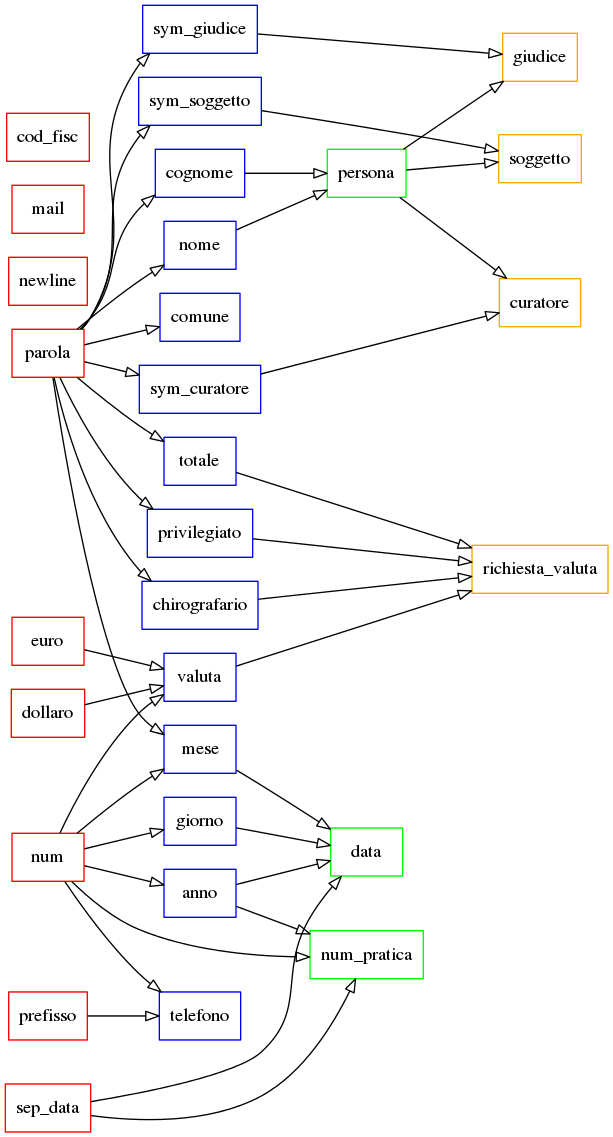
\includegraphics[width=.8\textwidth]{img/dipendenze.png}
\label{fig:dipendenze}
\caption[Dipendenze tra tag]{Schema delle dipendenze esistenti tra tag}
\end{figure}

In figura \ref{fig:dipendenze}, in \verb|tag| di colore rosso rappresentano il livello più basso, cioè i \verb|tag| riconoscibili a partire dai \verb|token| tramite analisi sintattica e espressioni regolari.

I \verb|tag| di colore blu utilizzano quelli del livello precedente per identificare nuove entità. Similmente succede per gli altri due livelli.

\subsubsection{Come funziona il tagger}

Similmente a quanto descritto a pagina \pageref{sec:creazionetoken} per i token, per ogni nuovo \verb|tag| viene creato un identificatore, nella forma \verb:tag<Num>: con \verb+<Num>+ intero positivo crescente.

Nell'ordine:
\begin{enumerate}
\item Viene asserito il nuovo tag tramite il predicato \verb|tag/2|;
\item Viene confermata l'appartenenza allo stesso documento dei \verb|token|/\verb|tag| dai quali deriva tramite il predicato \verb|appartiene/2|;
\item si asserisce la vicinanza (predicato \verb|next/2|) tra tutti i \verb|token|/\verb|tag| che precedono quelli dai quali deriva il \verb|tag| corrente e il \verb|tag| corrente;
\item si asserisce la vicinanza (predicato \verb|next/2|) tra il \verb|tag| corrente e tutti i \verb|token|/\verb|tag| che succedono a quelli dai quali deriva il \verb|tag| corrente;
\end{enumerate} 

Il codice seguente esemplifica alcune delle asserzioni del tagger in un documento composto da due parole: ``curatore fallimentare''.

\begin{prologcode}
token(tok0, BOF).
token(tok1, curatore).
token(tok2, fallimentare).
token(tok3, EOF).

tag(tag0, parola(curatore)).
next(tok0, tag0).
next(tag0, tok2).

tag(tag1, parola(fallimentare)).
next(tok1, tag1).
next(tag0, tag1).
next(tag1, tok3).
\end{prologcode}

La figura seguente invece, mostra invece tutti gli archi \verb|next| che vengono creati nel tagging di un documento composto dalle parole: ``Luigi Nesta''.

\begin{figure}[H]
\centering
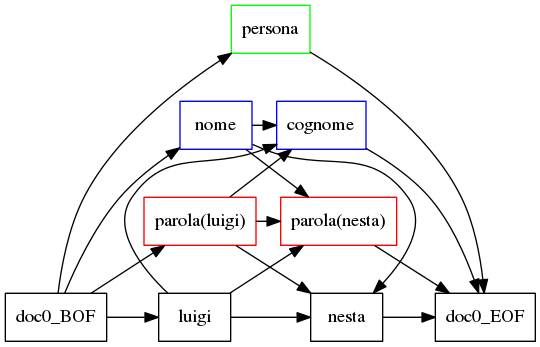
\includegraphics[width=\textwidth]{img/nuovitag.png}
\label{fig:nuovitag}
\caption[Esempio di ``next'']{Schema dei \emph{next/2} in un documento composto dalle parole ``Luigi Nesta''.}
\end{figure}
